%!TEX root = ../thesis_a4.tex

\chapter{Music Genre Classification Using Linear Models}
\label{sec:text-class}

\section{Introduction}
\label{sec:text-class:introduction}

%% INTRO PARAGRAPH TO CONNECT WITH CONTRIBUTIONS
%With the democratisation of Internet access, vast amounts of information are generated and stored in online sources, and thus there is great interest in developing techniques for processing this information effectively \cite{RuizCasadoetal2008}. The Music Information Retrieval (MIR) community is sensible to this reality, as music consumption has undergone significant changes recently, %\cite{Oramas2015}, 
%especially since users are today just one click away from millions of songs \cite{CelmaandHerrera2008}. This context results in the existence of large repositories of unstructured knowledge, which have great potential %as training data for Machine Learning (ML) algorithms, 
%for musicological studies or tasks within MIR such as music recommendation. 
%While there is substantial availability of textual data on one hand, and acoustic data, on the other, there is scarce work that explicitly addresses the interaction between them in multimodal datasets, let alone exploring their application to enhancing MIR, on one hand, or as evidence for studying musical trends, on the other.

In this chapter, we put forward an integration procedure for enriching with music-related information a large dataset of Amazon customer reviews \cite{McAuley2015a,McAuley2015}, with semantic and acoustic metadata obtained from MusicBrainz\footnote{\url{http://musicbrainz.org/}} and AcousticBrainz\footnote{\url{http://acousticbrainz.org}}, respectively. MusicBrainz (MB) is a large open music encyclopedia of music metadata, whilst AcousticBrainz (AB) is a database of music and audio descriptors, computed from audio recordings via state-of-the-art Music Information Retrieval algorithms \cite{Porter2015}.
In addition, we further extend the \textit{semantics} of the textual content from two standpoints. First, we apply an aspect-based sentiment analysis framework \cite{DongSOS13} which provides specific sentiment scores for different aspects present in the text, e.g. album cover, guitar, voice or lyrics. Second, we perform Entity Linking (EL), so that mentions to named entities such as Artist Names or Record Labels are linked to their corresponding Wikipedia entry \cite{Oramas2016}.

This enriched dataset, henceforth referred to as Multimodal Album Reviews Dataset (MARD), includes affective, semantic, acoustic and metadata features. % such as album release date.
We benefit from this multidimensional information to carry out two experiments. First, we explore the contribution of such features to the Music Genre classification task, consisting in, given a song or album review, predict the genre it belongs to. %This information can be used for Knowledge Graph generation and population, and thus has applications in Music Recommendation, Automatic Playlist Generation, and so forth. 
Second, we use the substantial amount of information at our disposal for performing a diachronic analysis of music criticism. Specifically, we combine the metadata retrieved for each review with their associated sentiment information, and generate visualizations to help us investigate any potential trends in diachronic music appreciation and criticism. Based on this evidence, and since music evokes emotions through mechanisms that are not unique to music \cite{Juslin2008}, we may go as far as using musical information as means for a better understanding of global affairs. Previous studies argue that national confidence may be expressed in any form of art, including music \cite{Moisi2010}, and in fact, there is strong evidence suggesting that our emotional reactions to music have important and far-reaching implications for our beliefs, goals and actions, as members of social and cultural groups \cite{Alcorta2008}. Our analysis hints at a potential correlation between the language used in music reviews and major geopolitical events or economic fluctuations. Finally, we argue that applying sentiment analysis to music corpora may be useful for diachronic musicological studies.


%% THIS PARAGRAPH SHOULD GO IN THE PLOTS SECTION
%A key point where changes in global mood and music perception met was 2008, a year in which according to research in geopolitics, ``the wall of racial prejudice fell as surely as the wall of oppression had fallen in Berlin twenty years earlier'' \cite{Moisi2010}. Our sentimental study reveals a much warmer and positive reaction towards genres easily associated with ethnic minorities in the US (latin music, jazz or R\&B), while other music genres like country or alternative rock received global minima in terms of affectiveness.

%\cite{Moisi2010}. 


%"music evokes emotions through mechanisms that are not unique to music" \cite{Juslin2008}"

%"In November 2008, at least for a time, hope prevailed over fear. The wall of racial prejudice fell as surely as the wall of oppression had fallen in Berlin twenty years earlier [...] Yet the emotional dimension of this election and the sense of pride it created in many Americans must not be underestimated."

%"national confidence may be expressed in architecture, art or music"



%Multimodal dataset: While textual data as well as acoustic data are available for the MIR community, they usually constitute one-dimensional products, as they often lack cross-modality intersection. For example, Amazon Review dataset is a well known collection of product reviews, which happens to include music products, but it is not enriched with Music-specific metadata and therefore for it to constitute a referential dataset for the MIR field it should further enriched with information from other dimensions. Likewise, there exist repositories of acoustic data available (freesound, Acousticbrainz? dontknow), or even manually curated structured Knowledge Bases in the Music domain such as MusicBrainz. In all the above cases, i.e. textual, acoustic and ontological, there is great room for improvement in terms integrating in one single dataset all this information. \textit{Add our contribution}. 

%Genre classification: While text classification is a well studied topic in Data Mining and Natural Language Processing, its potential as a key contributor to MIR remains to be fully explored. In addition, novel advances in NLP tasks like Sentiment Analysis or the exploitation of semantic properties via word embeddings have redefined certain tasks and hence the potential for advancing state-of-the-art classification algorithms has increased substantially. \textit{If its enough justified, add our contribution}.

%Studies on Music Criticism: The advent of the Big Data era opened up vibrant areas for Data Analytics, Data Mining and Machine Learning. Moreover, having such large scale information, often over long time series, enables studies on the Social Sciences side for the understanding of trends and perception of certain affairs, products or public personalities. We leverage the massive Amazon Product Dataset along with a Sentiment Analysis Framework (cite) in order to analyze diachronically the evolution of the language used in music criticism over time. A qualitative analysis of this analysis suggests that the overall perception of certain music genres may be influenced by major geopolitical events. \textit{Expand this contribution if needed}.

%\begin{itemize}
%    \item Release of a multimodal dataset of music albums with customer reviews, metadata and song audio descriptors.
%    \item Comparative of different approaches for genre classification, i.e. audio-based and text-based.
%    \item Proposal of a new methodology for systematic evolutionary studies on music criticism.
%\end{itemize}


\section{Multimodal Album Reviews Dataset}\label{sec:dataset}

MARD contains texts and accompanying metadata originally obtained from a much larger dataset of Amazon customer reviews \cite{McAuley2015a,McAuley2015}. The original dataset provides millions of review texts together with additional information such as overall rating (between 0 to 5), date of publication, or creator id. Each review is associated to a product and, for each product, additional metadata is also provided, namely Amazon product id, list of similar products, price, sell rank and genre categories. From this initial dataset, we selected the subset of products categorized as \textit{CDs \& Vinyls}, which also fulfill the following criteria. First, considering that the Amazon taxonomy of music genres contains 27 labels in the first hierarchy level, and about 500 in total, we obtain a music-relevant subset and select 16 of the 27 which really define a music style and discard for instance region categories (e.g. World Music) and other categories non specifically related to a music style (e.g. Soundtrack, Miscellaneous, Special Interest), function-oriented categories (Karaoke, Holiday \& Wedding) or categories whose albums might also be found under other categories (e.g. Opera \& Classical Vocal, Broadway \& Vocalists). We compiled albums belonging only to one of the 16 selected categories, i.e. no multiclass. Note that the original dataset contains not only reviews about CDs and Vinyls, but also about music DVDs and VHSs. Since these are not strictly speaking music audio products, we filter out those products also classified as "Movies \& TV". Finally, since products classified as Classical and Pop are substantially more frequent in the original dataset, we compensate this unbalance by limiting the number of albums of any genre to 10,000. After this preprocessing, MARD amounts to a total of 65,566 albums and 263,525 customer reviews. A breakdown of the number of albums per genre is provided in Table~\ref{tbl:dataset}.

%This dataset is formed by texts and metadata coming from Amazon costumers reviews from the "CDs \& Vinyls" section. It is a subset of a large dataset of costumer reviews gathered in \cite{McAuley2015a,Mauch150081}. Review texts come with some extra information , i.e. overall rating, date of publication and creator id. Every review is related to a music album. For every album there is also some attached information, i.e. title, Amazon product id, list of similar products, price, sell rank and genre categories. From the initial dataset, we selected those products that fulfill the following criteria. The Amazon taxonomy of genres has 27 genres in the first hierarchy level, and more than 500 in total. From the 27 categories, we selected 16 define a music style, and not a region (e.g. Asian music) or another classification criteria (e.g. Soundtrack). We selected albums that are classified into only one of 16 selected categories. The original dataset has not only reviews about CDs and Vinyls, but also music DVDs and VHSs. Hence, to focus only on audio products, we filter out products that were also categorized as "Movies \& TV" or were ranked in the Video sales ranking. In the original dataset, there is a higher predominance of products classified as Classical and Pop. To compensate that, we limited the number of albums of these genres to 10,000 in the final dataset. After the filtering process we kept a total of 65,566 albums and 263,525 customer reviews, which comprises the core of our dataset. The amount of albums by genre is shown in Table~\ref{tbl:dataset}.

\begin{table}[h]
\scriptsize
\centering
\begin{tabular}{|l|r|r|r|}
\hline
\textbf{Genre} & \textbf{Amazon} & \textbf{MusicBrainz} & \textbf{AcousticBrainz} \\
\hline
Alternative Rock & 2,674 & 1,696 & 564 \\
Reggae & 509 & 260 & 79 \\
Classical & 10,000 & 2,197 & 587 \\
R\&B & 2,114 & 2,950 & 982 \\
Country & 2,771 & 1,032 & 424 \\
Jazz & 6,890 & 2,990 & 863 \\
Metal & 1,785 & 1,294 & 500 \\
Pop & 10,000 & 4,422 & 1701 \\
New Age & 2,656 & 638 & 155 \\
Dance \& Electronic & 5,106 & 899 & 367 \\
Rap \& Hip-Hop & 1,679 & 768 & 207 \\
Latin Music & 7,924 & 3,237 & 425 \\
Rock & 7,315 & 4,100 & 1482 \\
Gospel & 900 & 274 & 33 \\
Blues & 1,158 & 448 & 135 \\
Folk & 2,085 & 848 & 179 \\
\hline
\textbf{Total} & 66,566 & 28,053 & 8,683 \\
\hline
\end{tabular}
\caption{Number of albums by genre with information from the different sources in MARD}
\label{tbl:dataset}
\end{table}

Having performed genre filtering, we enrich MARD by extracting artist names and record labels from the Amazon product page. We pivot over this information to query the MB search API to gather additional metadata such as release id, first release date, song titles and song ids. Mapping with MB is performed using the same methodology described in \cite{Oramas2015b}, following a pair-wise entity resolution approach based on string similarity with a threshold value of $\theta=0.85$. We successfully mapped 28,053 albums to MB. Then, we retrieved songs' audio descriptors from AB. From the 28,053 albums mapped to MB, a total of 8,683 albums are further linked to their corresponding AB entry, which encompasses 65,786 songs. The final dataset is freely available for download\footnote{http://mtg.upf.edu/download/datasets/mard}.
%Note that this is the number of songs present in AB at the time of the dataset creation, however, AB is continuously growing and more albums from the total mapped to MB might be also found in the future in AB. %A summary of the properties of our dataset and the interplay of the three resources is shown in Figure \ref{fig:dataset}, using the album ``The Adventures of Rick Slick'' (Rick Slick) as an example.

%\begin{figure}[!h]
%  \centering
%	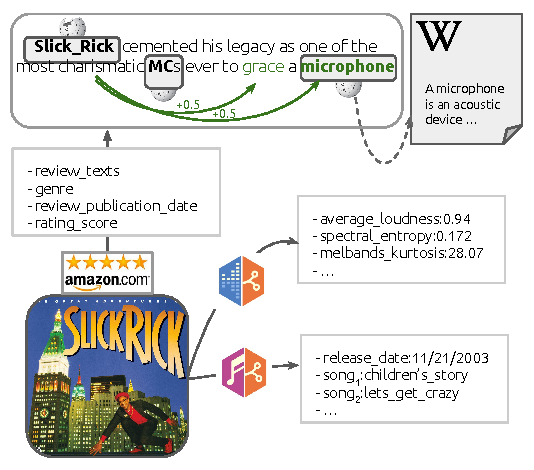
\includegraphics[width=8cm,height=7.25cm]{ch07_text-class/pics/dataset}
%  \caption{Summary of enrichment for every album review in our dataset, containing ontological (MB) and acoustic (AB) information as well as textual semantics.}
%  \label{fig:dataset}
%\end{figure}

%Once this genre-wise filtering was performed, we enrich the original ADR with artist name and record label. retrieved some extra information from Amazon that was not included in the original dataset, i.e. artist name and record label. Using the artist name and the album title we queried the MusicBrainz search API to try to gather more metadata about the albums, i.e. release group MBID (MusicBrainz ID), first release date, song titles and song MBID. For the mapping with MusicBrainz we followed a methodology similar to the one described in \cite{Flabase}. From the filtered set of albums, we obtained a mapping with MusicBrainz of 28,053 albums. Having the  MBIDs of the album songs, we can retrieve their audio descriptors present in AcousticBrainz. AcousticBrainz is a database of music descriptors computed from audio recordings using a number of state-of-the-art Music Information Retrieval algorithms. From the albums mapped to MusicBrainz, we found 8,683 albums for which their song descriptors were stored in AcousticBrainz. Audio descriptors of a total number of 65,786 songs were retrieved from AcousticBrainz.


\section{Text Processing}

In this section we describe how we extract linguistic, sentimental and semantic information from textual reviews. This information will serve both as input features for our genre classification experiments, and also constitute the basis for the diachronic study described in Section \ref{sec:evolution}.

\subsection{Sentiment Analysis}\label{sec:sentiment}
\begin{figure}
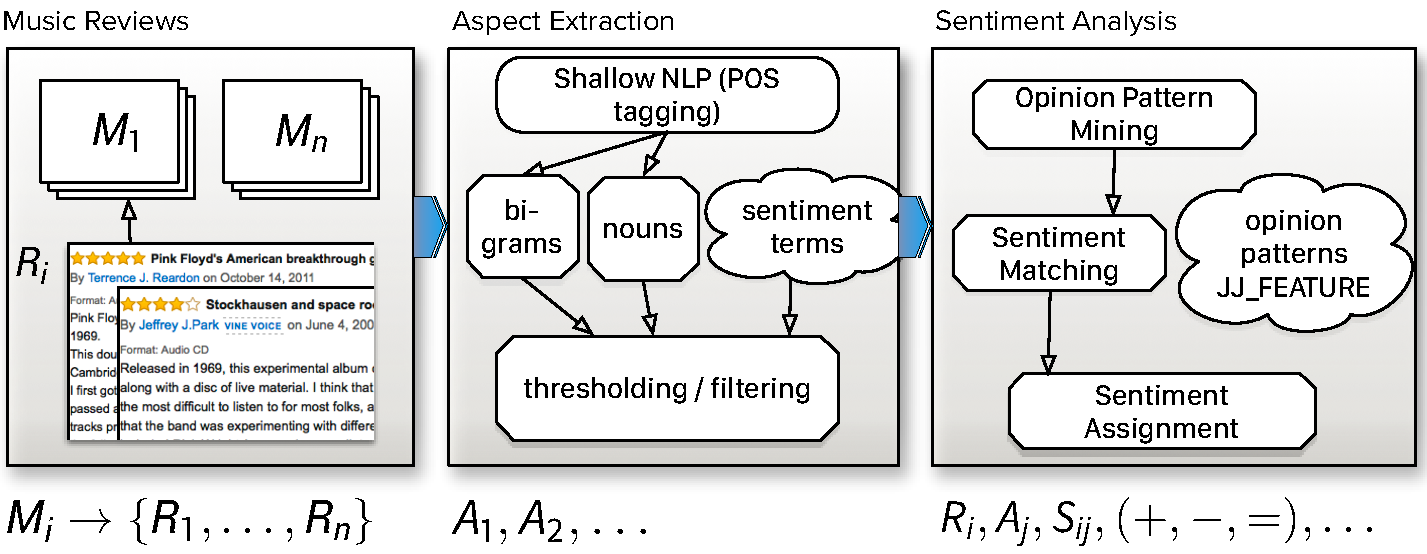
\includegraphics[width=\columnwidth]{ch07_text-class/pics/omf}
\caption{Overview of the opinion mining and sentiment analysis framework.}
\label{fig:OMF}
\end{figure}
Following the work of \cite{DongSOS13,DongOS14} we use a combination of shallow NLP, opinion mining, and sentiment analysis to extract opinionated features from reviews. For reviews $R_{i}$ of each album, we mine bi-grams and single-noun aspects (or review features), see \cite{Hu2004}; e.g. bi-grams which conform to a noun followed by a noun (e.g. \emph{chorus arrangement}) or an adjective followed by a noun (e.g. \emph{original sound}) are considered, excluding bi-grams whose adjective is a sentiment word (e.g. \emph{excellent}, \emph{terrible}). Separately, single-noun aspects are validated by eliminating nouns that are rarely associated with sentiment words in reviews, since such nouns are unlikely to refer to item aspects. We refer to each of these extracted aspects $A_{j}$ as review aspects.

For a review aspect $A_{j}$ we determine if there are any sentiment words in the sentence containing $A_{j}$. If not, $A_{j}$ is marked neutral, otherwise we identify the sentiment word $w_{min}$ with the minimum word-distance to $A_j$. Next we determine the POS tags for $w_{min}$, $A_i$ and any words that occur between $w_{min}$ and $A_i$. 
%This POS sequence is an opinion pattern. We compute the frequency of all opinion patterns in all reviews; a pattern is valid if it occurs more than average. For valid patterns, we assign sentiment score between -1 and 1 to $A_j$ based on the sentiment of $w_{min}$ and subject to whether the corresponding sentence contains any negation terms within $4$ words of $w_{min}$. 
We assign a sentiment score between -1 and 1 to $A_j$ based on the sentiment of $w_{min}$, subject to whether the corresponding sentence contains any negation terms within $4$ words of $w_{min}$. If there are no negation terms, then the sentiment assigned to $A_j$ is that of the sentiment word in the sentiment lexicon; otherwise this sentiment is reversed. Our sentiment lexicon is derived from SentiWordNet \cite{esuli2006sentiwordnet} and is not specifically tuned for music reviews.
%If an opinion pattern is not valid then we assign a neutral sentiment to each of its occurrences within the review set; see \cite{Moghaddam2010} for a more detailed description. 
An overview of the process is shown in Figure~\ref{fig:OMF}. The end result of sentiment analysis is that we determine a sentiment label $S_{ij}$ for each aspect $A_j$ in review $R_i$. A sample annotated review is shown in Figure~\ref{fig:annotatedreview}
\begin{figure}[h]
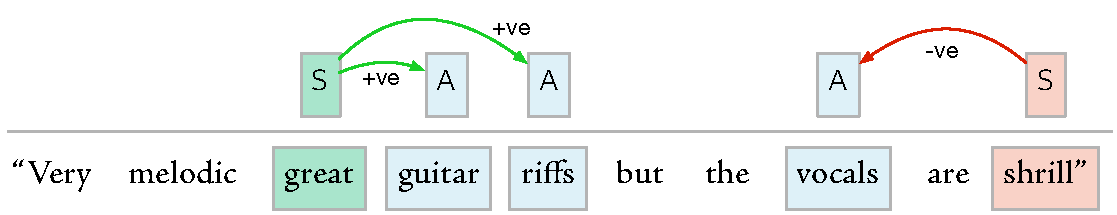
\includegraphics[width=\columnwidth]{ch07_text-class/pics/annotation_sample2}
\caption{A sentence from a sample review annotated with opinion and aspect pairs.}
\label{fig:annotatedreview}
\end{figure}

%Following the work of \cite{DongSOS13,DongOS14} we use a combination of shallow NLP, opinion mining, and sentiment analysis to extract opinionated features from reviews. For reviews $R_{i}$ of each album $A$, we mine bi-grams and single-noun aspects (or review features); see \cite{Hu2004,JustesonK95}; e.g. bi-grams which conform to a noun followed by a noun (e.g. \emph{chorus arrangement}) or an adjective followed by a noun (e.g. \emph{original sound}) are considered, excluding bi-grams whose adjective is a sentiment word (e.g. \emph{excellent}, \emph{terrible}). Separately, single-noun aspects are validated by eliminating nouns that are rarely associated with sentiment words in reviews, since such nouns are unlikely to refer to item aspects. We refer to each of these extracted aspects $A_{i}$ as review aspects.
%For a review aspect $A_{i}$ we determine if there are any sentiment words in the sentence containing $A_{i}$. If not, $A_{i}$ is marked neutral, otherwise we identify the sentiment word $w_{min}$ with the minimum word-distance to $A_i$. Next we determine the POS tags for $w_{min}$, $F_i$ and any words that occur between $w_{min}$ and $F_i$. This POS sequence is an opinion pattern. We compute the frequency of all opinion patterns in all reviews; a pattern is valid if it occurs more than average. For valid patterns, we assign sentiment score between -1 and 1 to $A_i$ based on the sentiment of $w_{min}$ and subject to whether the corresponding sentence contains any negation terms within $4$ words of $w_{min}$. If there are no negation terms, then the sentiment assigned to $A_i$ is that of the sentiment word in the sentiment lexicon; otherwise this sentiment is reversed. If an opinion pattern is not valid then we assign a neutral sentiment to each of its occurrences within the review set; see \cite{Moghaddam2010} for a more detailed description. An overview of the process is shown in Figure~\ref{fig:OMF}. The end result of sentiment analysis is that we determine a sentiment label $S_{ik}$ for each aspect $A_i$ in review $R_j$. A sample annotated review is shown in Figure~\ref{fig:annotatedreview}


\subsection{Entity Linking}\label{sec:disambiguation}

Entity Linking (EL) is the task to provide, given a mention to a named entity (e.g. person, location or organization), its most suitable entry in a reference Knowledge Base (KB) \cite{Moroetal2014b}. %This term is used to embody similar subtasks such as Named Entity Disambiguation, which is precisely linking mentions to entities to a KB.%, or Wikification \cite{MihalceaandCsomai2007}, i.e. performing Named Entity Disambiguation specifically against Wikipedia URIs.
In our case, EL was performed taking advantage of Tagme\footnote{http://tagme.di.unipi.it/} \cite{Ferragina2012}, an EL system that matches entity candidates with Wikipedia links, and then performs disambiguation exploiting both the in-link graph and the Wikipedia page dataset. %Then, it performs a pruning process by looking at the entity context. 
TagMe provides for each detected entity, its Wikipedia page id and Wikipedia categories.

\begin{table*}[]
\centering
\scriptsize
\begin{tabular}{|l|r|r|r|r|r|r|r|r|r|r|r|r|r|}
\hline
& Alt. Rock & Classical & Country & Electronic & Folk & Jazz & Latin & Metal & New Age & Pop & R\&B & Hip-Hop & Rock  \\
\hline
Alt. Rock & 28 / 42 & 1 / 3 & 3 / 1 & 10 / 10 & 7 / 1 & 1 / 2 & 2 / 0 & 18 / 12 & 10 / 2 & 4 / 10 & 3 / 6 & 3 / 2 & 10 / 9 \\
Classical & 0 / 0 & 87 / 95 & 1 / 0 & 0 / 0 & 1 / 1 & 1 / 1 & 2 / 2 & 1 / 0 & 5 / 1 & 1 / 0 & 0 / 0 & 0 / 0 & 1 / 0 \\
Country & 2 / 1 & 0 / 0 & 51 / 84 & 3 / 0 & 9 / 1 & 9 / 0 & 3 / 0 & 0 / 1 & 3 / 0 & 8 / 8 & 6 / 4 & 1 / 0 & 5 / 1 \\
Electronic & 7 / 3 & 3 / 1 & 1 / 2 & 40 / 61 & 4 / 1 & 1 / 2 & 2 / 2 & 6 / 0 & 7 / 5 & 6 / 5 & 6 / 7 & 13 / 5 & 4 / 7 \\
Folk & 4 / 6 & 11 / 0 & 13 / 10 & 7 / 0 & 27 / 55 & 6 / 1 & 7 / 3 & 4 / 2 & 6 / 9 & 5 / 9 & 6 / 4 & 1 / 0 & 3 / 1 \\
Jazz & 7 / 0 & 10 / 1 & 6 / 2 & 2 / 2 & 5 / 0 & 45 / 82 & 6 / 3 & 3 / 0 & 8 / 2 & 3 / 5 & 4 / 1 & 1 / 1 & 0 / 1 \\
Latin & 4 / 3 & 6 / 4 & 9 / 2 & 1 / 2 & 5 / 1 & 10 / 2 & 28 / 78 & 3 / 0 & 6 / 2 & 11 / 4 & 7 / 2 & 5 / 0 & 5 / 0 \\
Metal & 13 / 5 & 1 / 0 & 1 / 1 & 2 / 2 & 1 / 0 & 0 / 1 & 1 / 0 & 63 / 87 & 1 / 0 & 1 / 0 & 3 / 1 & 1 / 0 & 12 / 3 \\
New Age & 9 / 2 & 7 / 6 & 9 / 0 & 7 / 4 & 10 / 10 & 9 / 2 & 7 / 6 & 3 / 3 & 15 / 53 & 10 / 7 & 6 / 1 & 2 / 1 & 6 / 5 \\
Pop & 6 / 2 & 9 / 1 & 10 / 2 & 9 / 2 & 5 / 3 & 9 / 2 & 5 / 2 & 2 / 0 & 7 / 1 & 19 / 73 & 7 / 6 & 2 / 2 & 10 / 5 \\
R\&B & 8 / 2 & 0 / 1 & 16 / 3 & 8 / 4 & 2 / 0 & 5 / 3 & 5 / 0 & 1 / 0 & 3 / 0 & 7 / 10 & 24 / 71 & 17 / 5 & 4 / 1 \\
Hip-Hop & 8 / 2 & 0 / 0 & 2 / 1 & 8 / 2 & 0 / 1 & 0 / 1 & 1 / 0 & 4 / 3 & 2 / 0 & 4 / 1 & 7 / 2 & 61 / 86 & 3 / 1 \\
Rock & 17 / 15 & 1 / 2 & 6 / 8 & 4 / 7 & 10 / 5 & 2 / 4 & 7 / 1 & 12 / 13 & 4 / 1 & 9 / 7 & 7 / 4 & 6 / 2 & 15 / 31 \\
\hline
\end{tabular}
\caption{Confusion matrix showing results derived from AB acoustic-based classifier/BoW+SEM text-based approach.}
\label{tbl:confusion}
\end{table*}


\section{Music Genre Classification}\label{sec:classification}

%In this section we describe the music genre classification experiment. First, we briefly describe the subset of MARD used for training and testing, and then we provide a description of the features used for this task.

\subsection{Dataset Description}

Starting from MARD, our purpose is to create a subset suitable for genre classification, including 100 albums per genre class. We enforce these albums to be authored by different artists, and that review texts and audio descriptors of their songs are available in MARD. Then, for every album, we selected audio descriptors of the first song of each album as representative sample of the album. From the original 16 genres, 3 of them did not have enough instances complying with these prerequisites (Reggae, Blues and Gospel). This results in a classification dataset composed of 1,300 albums, divided in 13 different genres, with around 1,000 characters of review per album.
%An album may have a number of reviews with different length each. For each album we selected a subset of its reviews and concatenated their texts. We aimed to limit the cumulative length of the selected reviews of each album to 1000 characters approximately, without cropping any reviews. Finally, the average length of text by album in the classification dataset is 649 characters.

\subsection{Features}
\label{sec:features}
\subsubsection{Textual Surface Features}
We used a standard Vector Space Model representation of documents, where documents are represented as bag-of-words (BoW) after tokenizing and stopword removal. All words and bigrams (sequences of two words) are weighted according to \textit{tf-idf} measure. 

\subsubsection{Semantic Features}

We enriched the initial BoW vectors with semantic information thanks to the EL step. Specifically, for each named entity disambiguated with Tagme, its Wikipedia ID and its associated categories are added to the feature vector, also with \textit{tf-idf} weighting. Wikipedia categories are organized in a taxonomy, so we enriched the vectors by adding one level more of broader categories to the ones provided by Tagme. Broader categories were obtained by querying DBpedia\footnote{\url{http://dbpedia.org}}.

%We enriched the initial BoW vectors with semantic information thanks to the EL step. The semantic feature vector of an album is conformed by a BoW model where instead of words, there are entity IDs and categories. For every entity detected by Tagme in the album texts, we added to BoW its correspondent Wikipedia ID and the Wikipedia categories associated to this entity. We applied the tfidf measure to the semantic features vector to compute a weight associated to every entity and category for each album.

\subsubsection{Sentiment Features} 

Based on those aspects and associated polarity extracted with the opinion mining framework, with an average number of aspects per review around 37, we follow \cite{Suero2014} and implement a set of sentiment features, namely:

\begin{itemize}
    \item Positive to All Emotion Ratio: fraction of all sentimental features which are identified as positive (sentiment score greater than 0). 
    %Ratio between the positive aspects and all the aspectes identified in the text. We consider an aspect as positive if it has an associated sentiment score greater than 0, and negative if it is below 0. 
    %This feature is given by:
    %\begin{equation}
    %    PosRatio = \frac{PosAspects}{PosAspectes + NegAspects}
    %\end{equation}
    \item Document Emotion Ratio: fraction of total words with sentiments attached. This feature captures the degree of affectivity of a document regardless of its polarity.
    %This feature is designed to capture the degree of affectivity (regardless of polarity) of a document. It is based on the ratio of identified aspects to all words in the document. 
    %\begin{equation}
    %    eRatio = \frac{TotalAspects}{TotalWords}
    %\end{equation}
    \item Emotion Strength: This document-level feature is computed by averaging sentiment scores over all aspects in the document.
    %Emotion Strength: This feature shows the average of the sentiment scores associated to all the identified aspects in a document
    \item F-Score\footnote{Not to be confused with the evaluation metric.}: This feature has proven useful for describing the contextuality/formality of language. It takes into consideration the presence of \textit{a priori} ``descriptive'' POS tags (nouns and adjectives), as opposed to ``action'' ones such as verbs or adverbs.
    
    %It is designed to capture the usage of certain informative part-of-speech categories by looking at their frequency $F$, as follows:
    %\begin{equation}
    %\begin{split}
    %    Fscore = 0.5 * ((nounF+adjF+prepF+artF) \\
%-(pronF+verbF+advF+intF) + 100)
    %\end{split}
    %\end{equation}
\end{itemize}

\subsubsection{Acoustic Features}

Acoustic features are obtained from AB. They are computed using Essentia\footnote{\url{http://essentia.upf.edu/}}. These encompass loudness, dynamics, spectral shape of the signal, as well as additional descriptors such as time-domain, rhythm, and tone \cite{Porter2015}.% For instance, rhythm descriptors refer to beat positions and BPM value, while tonal information includes chroma features, keys and scales .

%Acoustic features, obtained from MB, are computed The set of acoustic features used is provided by AcousticBrainz, which is described in \cite{Porter2015}. These features are computed using the Essentia library\footnote{\url{http://essentia.upf.edu/}}. They are divided into low-level and high-level features. Low-level features encompasses spectral, time-domain, rhythm, and tonal descriptors, whilst high-level are generated after applying data mining and machine learning techniques over low-level features. We only used in our experiments the set of low-level features, which includes features characterizing overall loudness, dynamics, and spectral shape of the signal, rhythm descriptors (including beat positions and BPM value), and tonal information (including chroma features, keys and scales).


\subsection{Baseline approaches}
\label{sec:baselines}
Two baseline systems are implemented. First, we implement the text-based approach described in \cite{Hu2005} for music review genre classification. In this work, a Na\"{i}ve Bayes classifier is trained on a collection of 1,000 review texts, and after preprocessing (tokenisation and stemming), BoW features based on document frequencies are generated.
The second baseline is computed using the AB framework for song classification \cite{Porter2015}. Here, genre classification is computed using  multi-class support vector machines (SVMs) with a one-vs.-one voting strategy. The classifier is trained with the set of low-level features present in AB. %The dataset is split 80-20\% for training and testing, and accuracy values are obtained after 5-fold cross validation. 
%The second baseline is the well known audio-based approach for genre classification described in \cite{Tzanetakis2002}. Their experiments are performed on the GTZAN dataset, consisting in 1,000 audio files categorized across 10 genres. Given that classification results using this approach are already present in AcousticBrainz, we directly computed the accuracy of these predictions in our dataset. % Al quitar la diferencia entre low y high level features arriba he quitado aqui la ref a high level features. Tampoco se lo que son, asi que si es importante habra q modificarlo.

%We used two different baseline approaches to compare the obtained results. First, we implemented the text-based approach described in \cite{Hu2006} for genre classification of music reviews. In this work, a Multinomial Naive Bayes classifier is applied to a dataset of 1,000 reviews. Review texts are tokenized and stemmized and then document frequency of word tokens is computed and used as feature weight of a bag-of-words vector. We trained and tested the apporach on our dataset of review texts.
%Second, the well known audio-based approach for genre classification described in \cite{Tzanetakis2002} is applied to our dataset. In this work, the classifier is applied to a dataset of 1000 audio files classified into 10 different genres, known as the GTZAN dataset. Given that classification results using this approach are already present in the set of high-level features of AcousticBrainz, we directly computed the accuracy of these predictions in our dataset.


\subsection{Experiments}

\begin{table}[]
\centering
\begin{tabular}{l|r|r|r|}
\cline{2-4}
                                       & \multicolumn{1}{l|}{BoW} & \multicolumn{1}{l|}{BoW+SEM} & \multicolumn{1}{l|}{BoW+SENT} \\ \hline
\multicolumn{1}{|l|}{Linear SVM}       & \textbf{0.629}           & \textbf{0.691}               & \textbf{0.634}                \\ \hline
\multicolumn{1}{|l|}{Ridge Classifier} & 0.627                    & 0.689                        & 0.61                          \\ \hline
\multicolumn{1}{|l|}{Random Forest}    & 0.537                    & 0.6                          & 0.521                         \\ \hline
\end{tabular}
\caption{Accuracy of the different classifiers}
\label{tbl:classifiers}
\end{table}

We tested several classifiers typically used for text classification, namely Linear SVM, Ridge Classifier and Nearest Centroid, using the implementations provided by the scikit-learn library\footnote{http://scikit-learn.org/}. Among them, Linear SVM has shown better performance when combining different feature sets (see Table~\ref{tbl:classifiers}). Therefore, we trained a Linear SVM classifier with L2 penalty over different subsets of the features described in Section \ref{sec:features}, which are combined via linear aggregation. Specifically, we combine the different feature sets into five systems, namely \textbf{BoW} (BoW), \textbf{BoW+Semantic} without broader categories (BoW+SEM), \textbf{BoW+Semantic Broader} with broader categories (BoW+SEMb), \textbf{BoW+Sentiment} (BoW+SENT) and \textbf{BoW+Semantic+Sentiment} (BoW+SEM+SENT). In this way, we aim at understanding the extent to which sentiment and semantic features (and their interaction) may contribute to the review genre classification task. Note that this chapter is focused on the influence of textual features in genre classification, and classification based on acoustic features is simply used as a baseline for comparison. A proper combination of acoustic and textual features in text classification is a challenging problem and would require a deeper study that is out of the scope of this chapter.
The dataset is split 80-20\% for training and testing, and accuracy values are obtained after 5-fold cross validation. 
%As for training and test splits, we first divide the dataset, for each genre, in 80\% for training and 20\% for evaluation, and apply 5-fold cross-validation. We report average numbers across the 5 folds.

\begin{figure}
    \centering
    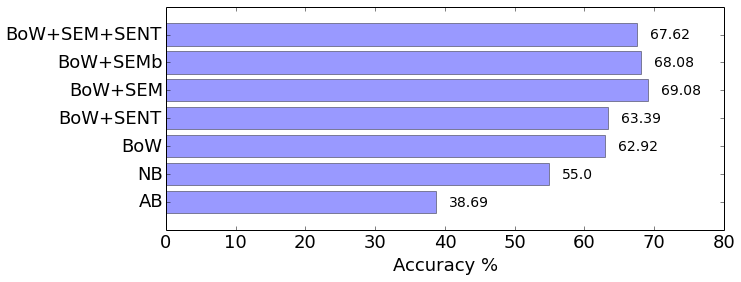
\includegraphics[width=\columnwidth]{ch07_text-class/pics/results2.png}
    \caption{Percentage of accuracy of the different approaches. AB refers to the AcousticBrainz framework. NB refers to the method based on Na\"{i}ve Bayes from \cite{Hu2005}.}
    \label{fig:results}
\end{figure}

%A comparison of the confusion matrix of the AcousticBrainz audio-based approach and the BoW+Sem text-based approach is shown in Table~\ref{tbl:confusion}. We observe that, although the text-based approach has higher accuracy in all the categories, both aporaches have a similar behaviour. This can explain why the combination of acoustic features with text-based features does not improve pure text-based approaches. We also note that both approaches have low accuracy values when distinguishing between Classic Rock and Alternative Rock. This means that the difference between these two categories is highly subtle, and neither acoustic nor text-based descriptors are able to properly help the classifier.


\subsection{Results and Discussion}

Accuracy results of the two baseline approaches introduced in Section \ref{sec:baselines} along with our approach variants are shown in Figure~\ref{fig:results}. At first sight, we may conclude that sentiment features contribute to slightly outperforming purely text-based approaches. This result implies that affective language present in a music review is not a salient feature for genre classification (at least with the technology we applied), although it certainly helps. On the contrary, semantic features clearly boost pure text-based features, achieving 69.08\% of accuracy. The inclusion of broader categories does not improve the results in the semantic approach. The combination of semantic and sentiment features improves the BoW approach, but the achieved accuracy is slightly lower than using semantic features only.%Although unreported due to space constraints, additional feature combinations were evaluated, considering for instance acoustic features, but their results were in general lower. 
% No creo que haga falta decir "lower than the systems in the figure bla", se sobreentiende no?

%Our aim in this experiment is to measure the impact of semantic and sentiment features in a text-based approach for genre classification. In addition, we want to compare these results with state-of-the-art audio-based approaches. The combination of acoustic and textual features is out of the scope of this chapter.
%The different approaches are built by linear aggregation of the different feature vectors. The approach used for genre classification is trained and tested on a Linear SVM classifier with L2 penalty. The dataset was split for each genre in 80\% for training and 20\% for testing. In addition, we applied 5-fold cross validation and averaged the results. Results of the three baseline approaches plus 3 text-based approaches with different combinations of features and are shown in Figure~\ref{fig:results}. We observe that sentiment features slightly outperforms a pure text-based approach. This result implies that measuring the positiveness or negativeness in the language used in a music review is not a salient feature for genre classification, although it certainly help. By contrast, semantic features really boost accuracy. The addition of external semantic information related to the entities present in the review help in the process of classification. We tried further combinations of features, including semantic, sentimental and acoustic features, but results did not improve the ones presented in Figure~\ref{fig:results}.

Let us review the results obtained with baseline systems. The Na\"{i}ve Bayes approach from \cite{Hu2005} is reported to achieve an accuracy of 78\%, while in our results it is below 55\%. The difference in accuracy may be due to the substantial difference in length of the review texts. In \cite{Hu2005}, review texts were at least 3,000 characters long, much larger that ours. Moreover, the addition of a distinction between Classic Rock and Alternative Rock is penalizing our results. 
As for the acoustic-based approach, although the obtained accuracy may seem low, it is in fact a good result for purely audio-based genre classification, given the high number of classes and the absence of artist bias in the dataset \cite{bogdanov2016cross}.
%As for the acoustic-based approach defined in \cite{Tzanetakis2002}, they achieve 61\% accuracy on the GZTAN dataset. However, certain bias in this dataset \cite{Sturm2012} may be responsible of such high performance. Therefore, we have taken the computation done in AcousticBrainz using this approach and trained on the GZTAN dataset to our dataset. As this approach classify a song among 10 different genres, and our dataset have 13 genres, we computed the average accuracy among the results only for this 10 genres. 
Finally, we refer to Table~\ref{tbl:confusion} to highlight the fact that the text-based approach clearly outperforms the acoustic-based classifier, although in general both show a similar behaviour across genres. Also, note the low accuracy for both Classic Rock and Alternative Rock, which suggests that their difference is subtle enough for making it a hard problem for automatic classification.

%We  did some trials at different character length, and this aspect revealed to be very determinant in the accuracy results. After performing several tests did some trials at different character length, and this aspect revealed to be very determinant in the accuracy results. In addition, the addition of a distinction between Classic and Alternative Rock is penalizing the results, as it has shown to be a difficult task. However, the aim of this experiment is compare different approaches among them, rather than achieving a very high value of accuracy.
%Furthermore, the acoustic-based approach defined in \cite{Tzanetakis2002} presents a result of 61\% of accuracy in the GZTAN dataset. However, some biases in the dataset \cite{Sturm2012} may be responsible of such a high level. Therefore, we have taken the computation done in AcousticBrainz using this approach and trained on the GZTAN dataset to our dataset. As this approach classify a song among 10 different genres, and our dataset have 13 genres, we computed the average accuracy among the results only for this 10 genres.

\section{Conclusions and Future Work}
In this work we have presented MARD, a multimodal dataset of album customer reviews combining text, metadata and acoustic features gathered from Amazon, MB and AB respectively. Customer review texts are further enriched with named entity disambiguation along with polarity information derived from aspect-based sentiment analysis. Based on this information, a text-based genre classifier is trained using different combinations of features. %Results are compared with an audio-based approach and a text-based approach. 
A comparative evaluation of features suggests that a combination of bag-of-words and semantic information has higher discriminative power, outperforming competing systems in terms of accuracy.
